\documentclass[12pt, a4paper]{article}

\usepackage[dvips]{graphics}
\usepackage{tabularx}
\usepackage{amsmath}
\usepackage{amsfonts}
\usepackage{amssymb}
\usepackage{graphicx}
\usepackage{float}
\usepackage{listings}
\usepackage{rotating}
\usepackage{tikz}
\usepackage{verbatim}
\usepackage{csvsimple}
\usepackage{rotating}
\usepackage{changepage}
\pdfgentounicode=1

\lstset{
        basicstyle=\ttfamily\scriptsize,
        keywordstyle=\bfseries,
        showspaces=false,
        showstringspaces=false,
        morekeywords={*,IF,FOR, STRUCT, FUNCTION, INT, FLOAT, ELSE, RETURN, STOP, Frame, FMB, PROJ, ELIM_VAR},
        mathescape=true
    }

\begin{document}

\title{The FMB algorithm}

\author{Pascal Baillehache}

\maketitle

\begin{center}
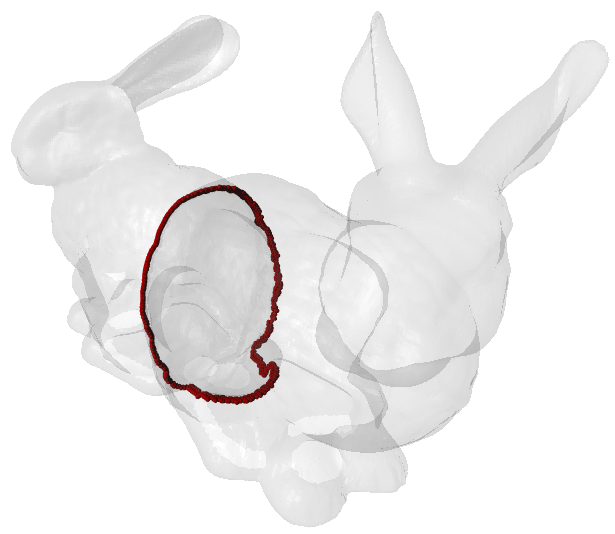
\includegraphics[width=2in]{bunny.png}\\
\label{fig:teaser}
\caption{Intersection detection on the Stanford Bunny,\\in 352s using FMB, 463s using SAT.}
\end{center}

\begin{abstract}
\small
This article introduces a simple and efficient algorithm to perform intersection detection on pairs of static/dynamic cuboid/tetrahedron in 2D and 3D using the Fourier-Motzkin elimination method. Qualification against the SAT algorithm shows that it is faster in the 3D static case, can be faster in the 3D dynamic case under conditions, and is slower in the 2D cases.
\end{abstract}

%-------------------------------------------------------------------------
\section{Introduction}
\label{sec:introduction}

Intersection detection of volumes is an ubiquitous problem in computer science: it is encountered in computer graphics, robotics, medical applications, entertainment, CAD for example. Considering the geometry of these volumes, the resolution of this problem ranges from straightforward to extremely difficult.

To overcome this difficulty, volumes are often approximated with simpler geometric shapes. These shapes are then used as bounding boxes to perform inaccurate but fast  detection, or as convenient representation of the orignal volumes on which efficient algorithms can be applied.

In this article I focus on the case of cuboids and tetrahedrons, which can be used either as Oriented Bounding Boxes or primitives for Volumetric Meshes, and the algorithms used to detect their intersection.

Commonly used algorithms in this case are SAT and CJK, based respectively on the Separating Axis Theorem and the Minkowski Difference. Another approach would be an algorithm based on the Fourier-Motzkin Elimination method. 

While such approach has been suggested in related work, no implementation and analysis of its performance could be found at the time of redaction. The aim of this article is to introduce an efficient representation of the intersection detection problem as a system of linear inequations, as well as an efficient algorithm based on Fourier-Motzkin Elimination to solve this particular system, and to check its performance by comparing it to SAT.

In the following sections, first I introduce related works to this article; then, I formulate the problem, explain how to solve it using the Fourier-Motzkin Elimination method, and introduce the FMB algorithm; finally, I give the validation and qualification results, and conclude by commenting them.

\section{Related Work}
\label{sec:relatedwork}

The SAT algorithm is based on the Separating Axis Theorem due to Minkowski. The details about the algorithm can be found in several sources, for example \emph{Geometric Tools for Computer Graphics} by Eberly and Schneider \cite{Eberly:2003}. Being another popular algorithm used to solve the same problem it has been selected to validate and qualify my work.

The Fourier-Motzkin Elimination method was introduced by Fourier \cite{Fourier:1827} and described by Motzkin \cite{Motzkin:1936}. Concerning its use to solve the problem of intersection detection, except for a suggestion by Ericson in \emph{Real-Time Collision Detection} \cite{Ericson:2005}, no detection algorithm using it could be found after investigation through several surveys \cite{Hornus:2015}\cite{Kunzler:2004}\cite{Jimenez:2001}\cite{Lin:1998}.

Ganovelli, Ponchio and Rocchini described the GPR algorithm in \emph{Fast Tetrahedron-Tetrahedron Overlap Algorithm} \cite{Ganovelli:2002}, based on a dimension reduction technique to improve the original SAT algorithm. Results show a significant improvement in performance for the Tetrahedron-Tetrahedron static case. FMB has been qualified on other cases too and achieves slightly better performances.

Imbert gave in \emph{About Redundant Inequalities Generated by Fourier's Algorithm} \cite{Imbert1990AboutRI} an improvement on the Fourier-Motzkin Elimination method to remove redundant inequations created during the resolution of the system. Its use in FMB has been considered before being discarded.

An alternative to the Fourier-Motzkin Elimination method to solve a system of linear inequations, also mentioned by Ericson \cite{Ericson:2005}, is the Seidel algorithm introduced in \emph{Linear Programming and Convex Hulls Made Easy} by Seidel \cite{Seidel:1990}. It is not covered by the work introduced in this article.

Another common algorithm for the intersection detection problem is the GJK algorithm due to Gilbert, Johnson and Keerthi \cite{Gilbert:1988}. It allows to calculate the distance between two convex sets but requires to have an efficient support function available for these sets. An implementation of GJK has been given by Cameron in \emph{Computing the Distance between Objects} \cite{Cameron:1996}.

About solving the more general problem of intersection detection on polyhedra, one can refer to \emph{Optimal detection of intersections between convex polyhedra} by Barba and Langerman \cite{Barba:2013}.

\section{Formulation of the problem}
\label{sec:formulation}

I formulate the intersection detection problem as a system of linear inequalities as described below, where I'm using the term \emph{Frame} to speak indifferently of Cuboids and Tetrahedrons in any dimension.

In a space of $D$ dimensions, I represent Frames as a set of $D+2$ vectors of dimension $D$: the origin vector $\vec{o}$, the velocity vector $\vec{v}$ and the $D$ component vectors $\vec{c_i}$. The volume of a Frame at instant $t$ can then be expressed as:
\begin{itemize}
\item for a Cuboid:
\end{itemize}
\begin{equation}
\left\lbrace\vec{o}+t\vec{v}+\sum_ix_i\vec{c_i}:x_i\in[0.0,1.0],i\in[1,D]\right\rbrace
\end{equation}
\begin{itemize}
\item for a Tetrahedron:
\end{itemize}
\begin{equation}
\begin{tabular}{c}
\left\lbrace\vec{o}+t\vec{v}+\sum_ix_i\vec{c_i}:x_i\in[0.0,1.0],\right.\\
\left.\sum_ix_i\le1.0,i\in[1,D]\right\rbrace$
\end{tabular}
\end{equation}
For convenience, I consider here a linear displacement at constant velocity over an interval of time represented by $t\in[0.0,1.0]$.

Given the pair of Frame $(A,B)$, the intersection detection problem is invariant with the coordinate system used. I can then project the pair $(A,B)$ into $A$'s own coordinate system. $A$'s representation becomes the standard basis in dimension $D$, and its velocity becomes $\vec{0}$. $B$'s representation becomes $\vec{o'}=\vec{o_B}-\vec{o_A}$, $\vec{v'}=\vec{v_B}-\vec{v_A}$ and its components $\vec{c'_i}$ are calculated by multiplication with the inverse matrix of $A$'s components.

This projection allows me to write the intersection volume, in $B$'s coordinate system, as:
\begin{itemize}
\item for a pair (Cuboid,Cuboid):
\end{itemize}
\begin{equation}
\left\lbrace\vec{x}:\vec{o'}+t\vec{v'}+\sum_ix_i\vec{c'_i}\in[0.0,1.0]^D,x_i\in[0.0,1.0],i\in[1,D]\right\rbrace
\end{equation}
\begin{itemize}
\item for a pair (Cuboid,Tetrahedron):
\end{itemize}
\begin{equation}
\begin{tabular}{c}
\left\lbrace\vec{x}:\vec{o'}+t\vec{v'}+\sum_ix_i\vec{c'_i}\in[0.0,1.0]^D,x_i\in[0.0,1.0],\right.\\
\left.\sum_ix_i\le1.0,i\in[1,D]\right\rbrace
\end{tabular}
\end{equation}
\begin{itemize}
\item for a pair (Tetrahedron,Cuboid):
\end{itemize}
\begin{equation}
\begin{tabular}{c}
\left\lbrace\vec{x}:\vec{o'}+t\vec{v'}+\sum_ix_i\vec{c'_i}\in[0.0,1.0]^D,x_i\in[0.0,1.0],i\in[1,D],\right.\\
\left.\sum_j\left(\vec{o'}+t\vec{v'}+\sum_ix_i\vec{c'_i}\right)_j\le1.0,j\in[1,D]\right\rbrace
\end{tabular}
\end{equation}
\begin{itemize}
\item for a pair (Tetrahedron,Tetrahedron):
\end{itemize}
\begin{equation}
\begin{tabular}{c}
\left\lbrace\vec{x}:\vec{o'}+t\vec{v'}+\sum_ix_i\vec{c'_i}\in[0.0,1.0]^D,x_i\in[0.0,1.0],i\in[1,D],\right.\\
\left.\sum_j\left(\vec{o'}+t\vec{v'}+\sum_ix_i\vec{c'_i}\right)_j\le1.0,\sum_ix_i\le1.0,j\in[1,D]\right\rbrace
\end{tabular}
\end{equation}

Finally, this leads to the following systems of linear inequations,
\begin{itemize}
\item for a pair (Cuboid,Cuboid):
\end{itemize}
\begin{equation}
\left\lbrace
\begin{array}{rcl}
t&\le&1.0\\
-t&\le&0.0\\
x_1&\le&1.0\\
...\\
x_D&\le&1.0\\
-x_1&\le&0.0\\
...\\
-x_D&\le&0.0\\
v'_1t+\sum_{i=1}^Dc'_{i,1}x_i&\le&1.0-o'_1\\
...\\
v'_Dt+\sum_{i=1}^Dc'_{i,D}x_i&\le&1.0-o'_D\\
-v'_1t-\sum_{i=1}^Dc'_{i,1}x_i&\le&o'_1\\
...\\
-v'_Dt-\sum_{i=1}^Dc'_{i,D}x_i&\le&o'_D
\end{array}
\right.
\end{equation}
\begin{itemize}
\item for a pair (Cuboid,Tetrahedron):
\end{itemize}
\begin{equation}
\left\lbrace
\begin{array}{rcl}
t&\le&1.0\\
-t&\le&0.0\\
-x_1&\le&0.0\\
...\\
-x_D&\le&0.0\\
v'_1t+\sum_{i=1}^Dc'_{i,1}x_i&\le&1.0-o'_1\\
...\\
v'_Dt+\sum_{i=1}^Dc'_{i,D}x_i&\le&1.0-o'_D\\
-v'_1t-\sum_{i=1}^Dc'_{i,1}x_i&\le&o'_1\\
...\\
-v'_Dt-\sum_{i=1}^Dc'_{i,D}x_i&\le&o'_D\\
\sum_{i=1}^Dx_i&\le&1.0
\end{array}
\right.
\end{equation}
\begin{itemize}
\item for a pair (Tetrahedron,Cuboid):
\end{itemize}
\begin{equation}
\left\lbrace
\begin{array}{rcl}
t&\le&1.0\\
-t&\le&0.0\\
x_1&\le&1.0\\
...\\
x_D&\le&1.0\\
-x_1&\le&0.0\\
...\\
-x_D&\le&0.0\\
-v'_1t-\sum_{i=1}^Dc'_{i,1}x_i&\le&o'_1\\
...\\
-v'_Dt-\sum_{i=1}^Dc'_{i,D}x_i&\le&o'_D\\
\sum_{j=1}^D\left(v'_jt+\sum_{i=1}^Dc'_{i,j}x_i\right)&\le&1.0-\sum_{j=1}^Do'_j
\end{array}
\right.
\end{equation}
\begin{itemize}
\item for a pair (Tetrahedron,Tetrahedron):
\begin{equation}
\left\lbrace
\begin{array}{rcl}
t&\le&1.0\\
-t&\le&0.0\\
-x_1&\le&0.0\\
...\\
-x_D&\le&0.0\\
-v'_1t-\sum_{i=1}^Dc'_{i,1}x_i&\le&o'_1\\
...\\
-v'_Dt-\sum_{i=1}^Dc'_{i,D}x_i&\le&o'_D\\
\sum_{i=1}^Dx_i&\le&1.0\\
\sum_{j=1}^D\left(v'_jt+\sum_{i=1}^Dc'_{i,j}x_i\right)&\le&1.0-\sum_{j=1}^Do'_j
\end{array}
\right.
\end{equation}

In static case, one can simply remove the elements related to $t$ from the systems.

\section{Resolution of the problem}
\label{sec:resolution}

The Fourier-Motzkin elimination method is a generalization of the Gaussian elimination method to linear systems of inequalities.

It consists of eliminating one variable of the system and rewrite a new system accordingly. Then the elimination operation is repeated on another variable in the new system, and so on until we obtain a trivial system with only one variable. From there, a solution for each variable can be obtained if it exists.

If the system has no solution, then there is no intersection between the two Frames. If the system has a solution, this is the bounding box of the intersection.

However, as far as one is only willing to detect intersection, one doesn't need to completely apply the method as only one inconsistent inequality is sufficient to prove the absence of intersection. Thus, one must check each inequality as soon as possible during the creation and resolution of the system to optimize the performance of the algorithm.

A sufficient condition for one inequality $\sum_ia_ix_i\le y$ to be inconsistent is, given the convenient property of the considered system $\forall i,x_i\in[0.0,1.0]$:
\begin{equation}
\label{eqn:cond_non_intersec}
y<\sum_{i\in \mathbb{I^-}}a_i
\end{equation}
where $\mathbb{I^-}=\left\lbrace i:a_i<0.0\right\rbrace$

Then, inequations with the highest probability of fulfilling Inequation~\ref{eqn:cond_non_intersec} should be processed first. Ideally, new inequations produced by the elimination method should be sorted on the decreasing values of $a_i$ and increasing values of $y$, but such operation would definitely be too much time consuming. Thus, only explicit sorting of the inequations in the initial system, and verification of the inconsistency condition for each new inequation, are performed in the FMB algorithm.

A drawback of the Fourier-Motzkin elimination method is the explosion in number of inequations in the system during its resolution, up to several hundreds for the 3D dynamic case. Some of these inequations are redundants and can be discarded without affecting the solution.

One way to detect redundant inequations is based on the following principle. Given $x\in[0.0,1.0]$, $a\in\mathbb{R^+}$, $b\in\mathbb{R}$, and the two inequations $ax<b$ and $a'x<b'$, then if $b/a<b'/a'$ the second one is redundant and can be removed from the system. This can be generalized to higher number of variables.

Reduction of the total number of inequations using this principle has successfully been implemented, leading to reduction by 15\% and 40\% in 2D and 3D static cases. Unfortunately, the extra cost of computation cancelled the gain despite various experimentations. Thus, it has been discarded.

The Imbert's acceleration theorem described in Imbert \cite{Imbert1990AboutRI} has also been discarded for the same reason. It is important to note however that if FMB were to be applied to much higher dimensions the balance may turn in favor of these optimization methods.

\section{Algorithm}
\label{sec:algorithm}

The generic version of the FMB algorithm is given in pseudo-code in Listing~\ref{lst:fmb}. One should take care to adapt this version according to its needs for better performance, for example by removing the [\lstinline{IF DYNAMIC CASE}] blocks when using the algorithm in static case, unwinding loops where possible, and using constant values where ever there are variables based on \lstinline{DIM}.

\begin{lstlisting}[breaklines, caption={The FMB algorithm.}, label={lst:fmb}]
DIM is the space dimension

STRUCT Frame
  FLOAT orig[DIM]
  FLOAT comp[DIM][DIM]    <- comp[i-th component][j-th axis]
  FLOAT invComp[DIM][DIM] <- inverse matrix of comp
  IF DYNAMIC CASE
    FLOAT speed[DIM]

FUNCTION FMB(Frame A, Frame B)
  Frame Ba := PROJ(A, B)
  INT nbVars := DIM
  IF DYNAMIC CASE
    nbVars := DIM + 1
  FLOAT M[][nbVars]
  FLOAT Y[]
  FOR j IN 0..DIM-1
    FOR i IN 0..DIM-1
      M[j][i] := -Ba.comp[i][j] 
    IF DYNAMIC CASE
      M[j][DIM] := -Ba.speed[j] 
    Y[j] := Ba.orig[j] 
    IF Y[j] < SUM OF NEGATIVE VALUES IN M[j][0..nbVars-1]
      A AND B ARE NOT INTERSECTING, STOP
  nbRows := DIM
  IF A IS A CUBOID
    FOR j IN 0..DIM-1
      FOR i IN 0..DIM-1
        M[nbRows][i] := Ba.comp[i][j] 
      IF DYNAMIC CASE
        M[nbRows][DIM] := Ba.speed[j] 
      Y[nbRows] := 1 - Ba.orig[j] 
      IF Y[nbRows] < 
          SUM OF NEGATIVE VALUES IN M[nbRows][0..nbVars-1]
        A AND B ARE NOT INTERSECTING, STOP
      nbRows := nbRows + 1
  ELSE
    FOR i IN 0..DIM-1
      M[nbRows][i] := SUM OF Ba.comp[i][0..DIM-1]
    IF DYNAMIC CASE
      M[nbRows][DIM] := SUM OF Ba.speed[0..DIM-1]
    Y[nbRows] = 1 - (SUM OF Ba.orig[0..DIM-1]) 
    IF Y[nbRows] < SUM OF NEGATIVE VALUES IN M[nbRows][0..nbVars-1]
      A AND B ARE NOT INTERSECTING, STOP
    nbRows := nbRows + 1
  IF B IS A CUBOID
    FOR j IN 0..DIM-1
      FOR i IN 0..nbVars-1
        IF i = j
          M[nbRows][i] := 1
        ELSE
          M[nbRows][i] := 0
      Y[nbRows] := 1
      nbRows := nbRows + 1
  ELSE
    FOR i IN 0..DIM-1
      M[nbRows][0] := 1 
    IF DYNAMIC CASE
      M[nbRows][DIM] := 0
    Y[nbRows] := 1 
    nbRows := nbRows + 1
  FOR j IN 0..DIM-1
    FOR i IN 0..nbVars-1
      IF i = j
        M[nbRows][i] := -1
      ELSE
        M[nbRows][i] := 0
    Y[nbRows] := 0
    nbRows := nbRows + 1
  IF DYNAMIC CASE
    FOR i IN 0..nbVars-1
      IF i = nbVars - 1
        M[nbRows][i] := 1
        M[nbRows+1][i] := -1
      ELSE
        M[nbRows][i] := 0
        M[nbRows+1][i] := 0
    Y[nbRows] := 1
    Y[nbRows+1] := 0
    nbRows := nbRows + 2
  FOR i IN 0..nbVars-2
    M, Y, nbRows := ELIM_VAR(M, Y, nbVars - i, nbRows)
  FLOAT bounds[2] := [0, 1]
  FOR i IN 0..nbRows-1
    IF M[i][0] > 0
      y := Y[i] / M[i][0]
      IF bounds[1] > y
        bounds[1] := y
    ELSE IF M[i][0] < 0
      y := Y[i] / M[i][0]
      IF bounds[0] < y
        bounds[0] := y
  IF bounds[0] >= bounds[1]
    A AND B ARE NOT INTERSECTING, STOP
  ELSE
    A AND B ARE INTERSECTING, STOP

FUNCTION PROJ(Frame A, Frame B)
  Frame Ba
  FLOAT v[DIM]
  IF NOT ALREADY COMPUTED
    A.invComp := INVERSE MATRIX OF A.comp
  IF DYNAMIC CASE
    FLOAT s[DIM]
  FOR i IN 0..DIM-1
    v[i] := B.orig[i] - A.orig[i] 
    IF DYNAMIC CASE
      s[i] := B.speed[i] - A.speed[i] 
  FOR i IN 0..DIM-1
    Ba.orig[i] := 0
    IF DYNAMIC CASE
      Ba.speed[i] := 0 
    FOR j IN 0..DIM-1
      Ba.orig[i] := Ba.orig[i] + A.invComp[j][i] * v[j] 
      IF DYNAMIC CASE
        Ba.speed[i] := Ba.speed[i] + A.invComp[j][i] * s[j] 
      Ba.comp[j][i] = 0 
      FOR k IN 0..DIM-1
        Ba.comp[j][i] :=
          Ba.comp[j][i] + A.invComp[k][i] * B.comp[j][k] 
  RETURN Ba

FUNCTION ELIM_VAR(FLOAT M[][], FLOAT Y[], INT nbVars, INT nbRows)
  INT nbRowsP := 0 
  FLOAT Mp[][nbVars-1]
  FLOAT Yp[]
  FOR iRow IN 0..nbRows-2
    IF M[iRow][0] <> 0
      FOR jRow IN iRow+1..nbRows-1
        IF M[jRow][0] <> 0 AND M[iRow][0] * M[jRow][0] < 0
          FOR iCol IN 1..nbCols-1
            Mp[nbRowsP][iCol-1] := 
              M[iRow][iCol] / ABS(M[iRow][0]) + 
              M[jRow][iCol] / ABS(M[jRow][0]) 
          Yp[nbRowsP] := 
            Y[iRow] / ABS(M[iRow][0]) +
            Y[jRow] / ABS(M[jRow][0]) 
          IF Yp[nbRowsP] < 
              SUM OF NEGATIVE VALUES IN Mp[nbRowsP][0..nbCols-2]
            A AND B ARE NOT INTERSECTING, STOP
          nbRowsP := nbRowsP + 1 
  FOR iRow IN 0..nbRows-1
    IF M[iRow][0] = 0
      FOR iCol IN 1..nbCols-1
        Mp[nbRowsP][iCol-1] := M[iRow][iCol] 
      Yp[nbRowsP] := Y[iRow] 
      nbRowsP := nbRowsP + 1 
  RETURN Mp, Yp, nbRowsP
\end{lstlisting}

\section{Results}

\subsection{Validation}

The validation procedure consisted of creating 1.000.000 random pairs of tetrahedron/cuboid for each case 2D/3D static/dynamic, then to perform an intersection detection on each pair A-B and its symmetric B-A using the SAT and FMB algorithms, and finally to check that the results were concordant between the two algorithms.

The validation procedure was successfull.

\subsection{Qualification}

The qualification procedure consisted of creating 500.000 random pairs of tetrahedron/cuboid for each case 2D/3D static/dynamic, then to perform an intersection detection on each pair A-B and its symmetric B-A using the SAT and FMB algorithms, and finally to calculate the ratio (execution time FMB) / (execution time SAT).

The average of these ratio are given in Table~\ref{tbl:ratio} (values below 1.0, in blue, means FMB is faster than SAT). Results are given here with the inversion of components' matrix computed during FMB for fairness against SAT which doesn't need it. But it may be in real use cases already available, improving results in favor of FMB. For example, as long as the components do not change (i.e. the Frame is undeformable and does not rotate) one can compute the inverse once for all and reuse it.

Execution environment for qualification was: operating system Ubuntu 18.04, processor Intel i7-8700T, implementation in C, compiler gcc version 7.5.0 using option -O3.

\begin{table}[htp]
\small
\begin{center}
\begin{tabular}{|c|c|c|c|c|c|c|c|}
\hline
 & \multicolumn{2}{|c|}{Cuboid-Cuboid} & \multicolumn{2}{|c|}{Cuboid-Tetrahedron} & \multicolumn{2}{|c|}{Tetrahedron-Tetrahedron}\\
\hline
 & inters. & no inters. & inters. & no inters. & inters. & no inters.\\
\hline
2D static & {\color[rgb]{1.0,0.0,0.0}2.58} & {\color[rgb]{1.0,0.0,0.0}1.22} & {\color[rgb]{1.0,0.0,0.0}1.86} & {\color[rgb]{1.0,0.0,0.0}1.29} & {\color[rgb]{1.0,0.0,0.0}1.33} & {\color[rgb]{1.0,0.0,0.0}1.32}\\
\hline
3D static & {\color[rgb]{0.0,0.0,1.0}0.72} & {\color[rgb]{0.0,0.0,1.0}0.50} & {\color[rgb]{0.0,0.0,1.0}0.41} & {\color[rgb]{0.0,0.0,1.0}0.66} & {\color[rgb]{0.0,0.0,1.0}0.24} & {\color[rgb]{0.0,0.0,1.0}0.89}\\
\hline
2D dynamic & {\color[rgb]{1.0,0.0,0.0}3.12} & {\color[rgb]{1.0,0.0,0.0}1.50} & {\color[rgb]{1.0,0.0,0.0}2.22} & {\color[rgb]{1.0,0.0,0.0}1.50} & {\color[rgb]{1.0,0.0,0.0}1.67} & {\color[rgb]{1.0,0.0,0.0}1.50}\\
\hline
3D dynamic & {\color[rgb]{1.0,0.0,0.0}2.58} & {\color[rgb]{0.0,0.0,1.0}0.71} & {\color[rgb]{1.0,0.0,0.0}1.37} & {\color[rgb]{0.0,0.0,1.0}0.81} & {\color[rgb]{0.0,0.0,1.0}0.54} & {\color[rgb]{0.0,0.0,1.0}0.95}\\
\hline
\end{tabular}
\end{center}
\caption{Ratio (execution time FMB) / (execution time SAT)}
\label{tbl:ratio}
\end{table}

\section{Conclusion}

In this article I've introduced the FMB algorithm, based on the Fourier-Motzkin elimination method, to solve the intersection detection problem of 2D/3D static/dynamic cuboid/tetrahedron.

Validation against the SAT algorithm proved its correctness. Qualification against the same showed it's, in term of average speed, a better alternative in the 3D static case. In the 3D dynamic case, it's also a better alternative when applied to pairs of Tetrahedrons. Depending on the ratio of pairs intersecting/not intersecting in the tested sets for other types of Frame the advantage varies between SAT and FMB. In 2D cases FMB is in average always slower than SAT.

The FMB algorithm is simple to implement, suitable to parallelization, and straightforward to adapt to higher dimensions or mesh faces in 3D. As it uses a data structure compatible with SAT, it can be easily integrated in an hybrid system taking advantage of both algorithms. Furthermore, FMB can give the bounding box of the intersection, if any, at very little extra cost.

It is also opened to further research, by looking for more efficient ways to restrain the number of inequations in the system, a stronger condition for the detection of inconsistency, hardware implementation, possible application to polyhedrons, etc.

\subsection*{Acknowledgements}
The author would like to express his gratitude to Mr Bornet and Mr Trotoux for their teaching, and Mr Ericson for his encouragement. The Stanford Bunny model was provided by the Stanford University Computer Graphics Laboratory.

\small
\bibliographystyle{unsrt}
\bibliography{article}

\section*{Supplemental Materials}
The C implementation of the FMB algorithm, the code used for validation and qualification, and the detailed results are provided at\\https://github.com/BayashiPascal/FMB/.

\section*{Author Contact Information}

\hspace{-2mm}\begin{tabular}{p{0.5\textwidth}p{0.5\textwidth}}
Pascal Baillehache \newline
bayashipascal@gmail.com
\end{tabular}

\end{document}
